\section{Region Based Object Detection} 

  So far, we have talked about classification, but this is fundamentally a different problem than object detection. Many aspects will be shared between the two problems. Essentially in detection algorithms, we try to draw a bounding box around the object of interest to locate it within the image. There could be many bounding boxes representing different objects of interest, and what makes this so challenging is that we don't know how many beforehand. Because of these bounding boxes, we must use models that predict also the number and the dimensions of these boxes, use datasets that provide these bounding boxes in addition to labels (e.g. COCO, VOC), and finally we must construct loss functions that take into consideration these boxes. 

  Therefore, the major reason why you cannot proceed with this problem by building a standard CNN followed by a fully connected layer is that the length of the output layer is variable. A naive approach to solve this problem would be to take different regions of interest from an image and use a CNN to classify the presence of the object within that region. That is, we do the following steps. 
  \begin{enumerate}
    \item We have an input image $\mathbf{x}$, and we want to define a set of subimages $\mathcal{R}$. Each element of $\mathcal{R}$ is essentially a box that segments out a portion of the image $\mathbf{x}$, and we can parameterize this box with 4 numbers. Two of the most popular ones is to take the center of the box plus the width and height $(c_x, c_y, w, h)$ or to take the top-left and bottom-right corners $(x_{min}, y_{min}, x_{max}, y_{max})$. Essentially, we have a giant set of vectors in $\mathbb{R}^4$, and each element is called a \textbf{region of interest}. 
    \item We now take each ROI and input this to our trusty CNN and do the classification task that we have studied up until now. This should tell us whether there is our object of interest in the image or not, and if it passes a certain threshold, we can have it infer that this ROI contains the object. If multiple ROIs pass the threshold, then we can pick the ROI for which the CNN outputs the highest probability of the object existing in.  
  \end{enumerate}

  This workflow essentially just extracts the regions of interest and does vanilla classification on them. This is an intuitive extension of what we know, but there are a few problems with this approach: 
  \begin{enumerate}
    \item A small problem is that the ROIs in $\mathcal{R}$ may not be the same size, while our CNN feature extractor requires its inputs to be fixed. However, this isn't too bad since we can just resize the ROIs for preprocessing. We could also just have $\mathcal{R}$ contain all images of the same size, but this will really hamper the robustness of the model. Objects can be of different size, and so intuitively, we must have different sized ROIs. 

    \item There is the bigger question of how we actually construct $\mathcal{R}$. We have a tradeoff. If $\mathcal{R}$ is too small, it may not capture the structure of the objects of interest. If it is too large, then we may have a combinatoral explosion of ROIs to look for. For example, if we simply have a sliding window with a stride of $1$ that adds each image into $\mathcal{R}$, for an $N \times N$ image we would have $O(N^2)$ ROIs, and this is only for one resolution! This may have been feasible if we were working with linear models, but in the deep learning regime this is not. This second problem is what we will focus on when explaining R-CNNs. 
    
      \begin{center}
        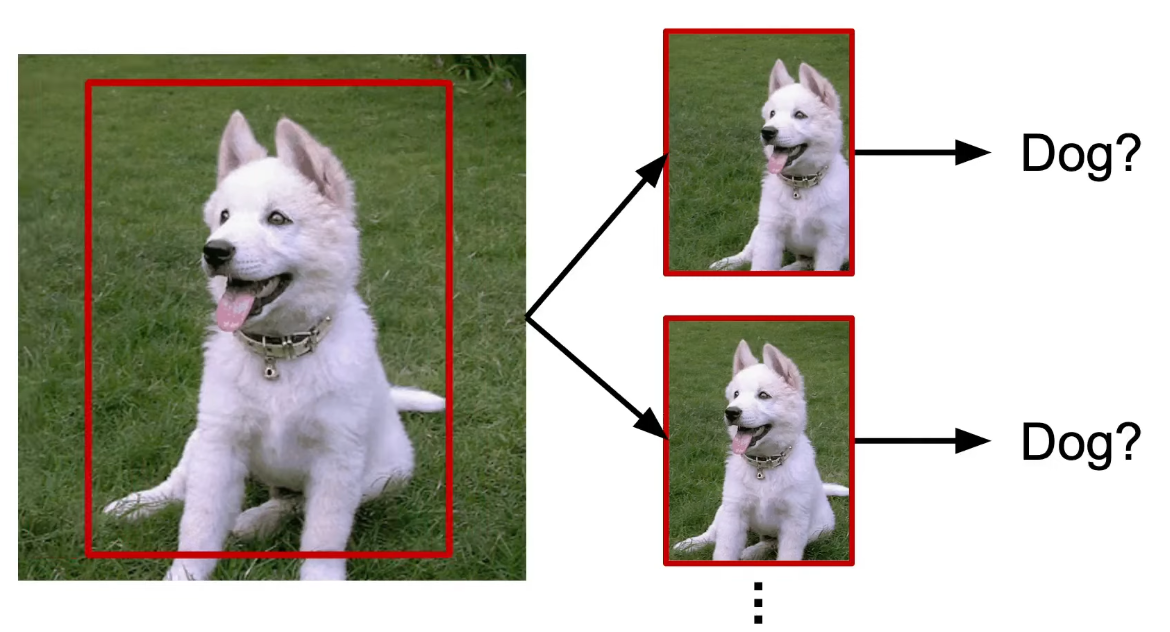
\includegraphics[scale=0.3]{img/sliding_window.png}
      \end{center}
  \end{enumerate}

\subsection{Region-Based CNN}

  The region-based CNN first bounds $|\mathcal{R}| \leq 2000$ and uses classical image processing techinques to reduce the number of ROIs to less than $2000$. 
  \begin{enumerate} 
    \item We start off by using the \textbf{selective search algorithm}. It over-segments the image into seed regions, with each region generating a bounding box. This leads to a ton of regions to look for, and to reduce $|\mathcal{R}|$, we use a greedy algorithm to recursively combine similar regions into larger ones. The segmentation algorithm is the basis of the region proposals, since it matches similar pixels together for a good intialization, giving us the best balance between computational feasibility and quality of proposals. It is specifically designed to have high recall, but low precision, which means that it returns many false positive regions, but are quite certain that they contain the objects of interest.  
      \begin{center} 
        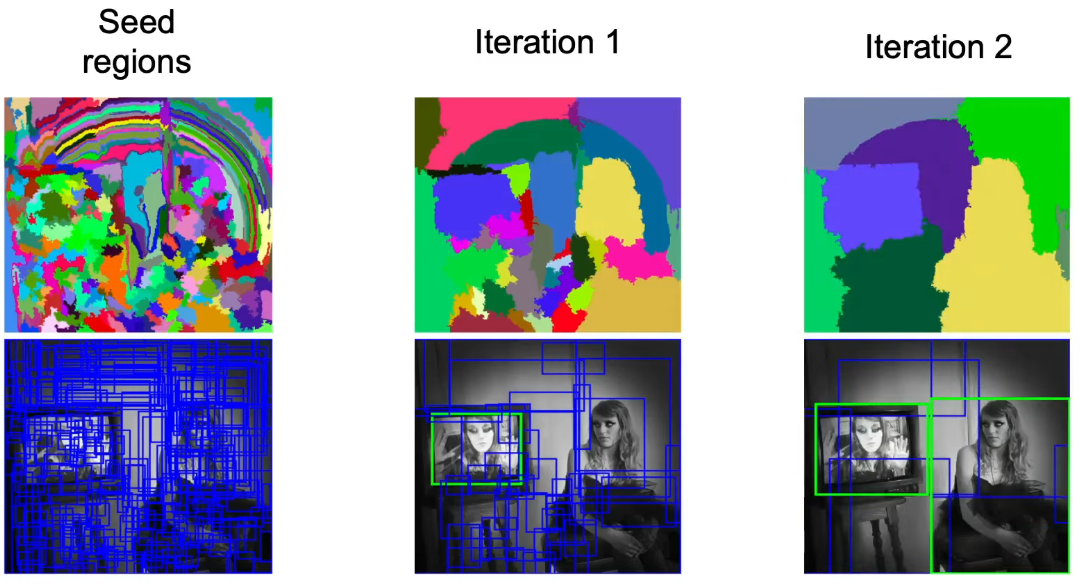
\includegraphics[scale=0.3]{img/selective_search.png} 
      \end{center}
    
    \item This usually leads to about 2000 ROIs, and for each ROI, we warp them into a square and feed them into a CNN, which produces a $4096$-dimensional feature vector as output. 

    \item The CNN acts as a feature extractor and the output dense layer consists of the feature extracted from the image. This $4096$-vector is fed into a support vector machine to classify the presence of the object within that candidate region proposal. 
      \begin{center}
        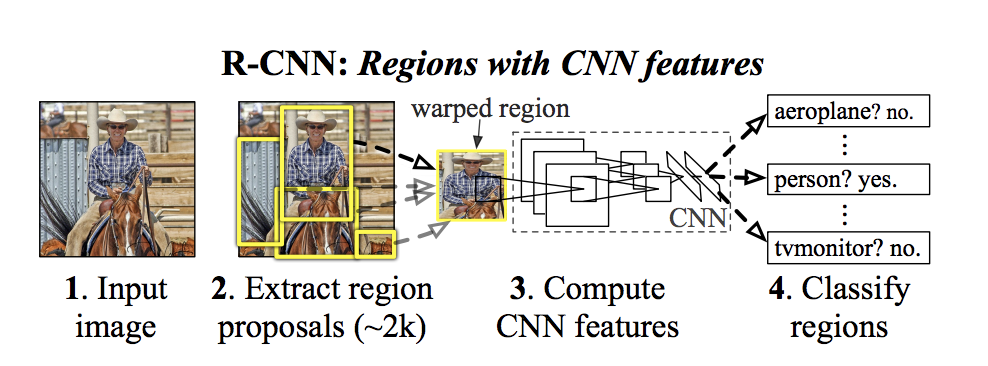
\includegraphics[scale=0.4]{img/rcnn_diagram.png}
      \end{center}

    \item In addition to predicting the presence of an object within the region proposals, the algorithm also predicts 4 values which are offset values to increase the precision of the bounding box. For example, given a region proposal, the algorithm would have predicted the presence of a person but the face of that person within that region proposal could have been cut in half. Therefore, these offset values can help in adjusting the bbox.  
      \begin{center}
        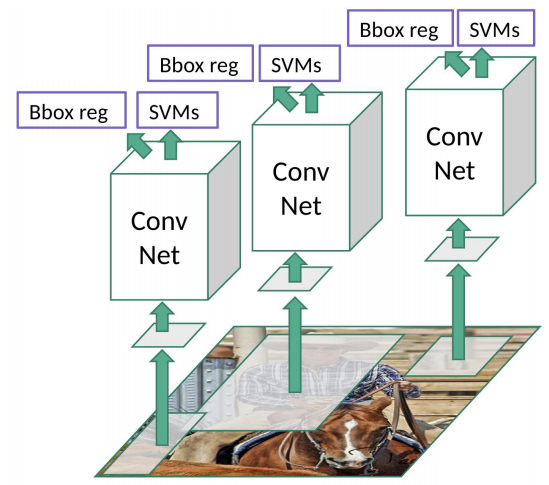
\includegraphics[scale=0.5]{img/rcnn_diagram2.png} 
      \end{center}
  \end{enumerate}

  However, there are still several problems: 
  \begin{enumerate}
      \item While we have improved the computational cost by a lot, we still have to run the CNN feature extractor on \textit{each} of the $2000$ region proposals, which is still too slow for real time inference (takes about 47 seconds), and it takes too long to train. 
      \item When we reshape each region proposal into a square, it may warp the image, causing it to lose its original features. 
      \item The selective search algorithm is not a learning algorithm, so it may generate bad candidate region proposals for various types of images.  
      \item Finally, the R-CNN model is not trained on an end-to-end fashion (the SVM) is trained separately, so this may reduce potential performance. 
  \end{enumerate} 

  \begin{definition}[IOU]
  To provide a measure of how good these boxes are, we use the \textbf{intersection over union (IOU)} metric. If $B$ is the true bounding box and $\Tilde{B}$ our estimate of it, then we have 
  \[\mathrm{IoU} = \frac{\mu(B \cap \Tilde{B})}{\mu(B \cup \Tilde{B})}\]
  The closer it is to $1$, the better, and a ``good" match is defined to be $0.7$ or above.  
  \end{definition} 

\subsection{Fast RCNN}

  Fast RCNN is basically just RCNN but with a few tweaks to make it fast. The computational bottleneck came from having to run a CNN on each of the 2000 region proposals, but now, to speed things up, we have a CNN extract features from the whole image first. We describe the steps below. 
  \begin{enumerate} 
    \item We take the image $\mathbf{x} \in \mathbb{R}^{n \times m}$ and use the CNN $f$ to extract features from it, resulting in say $\boldsymbol{\phi} \in \mathcal{F}$.
    \item At the same time, we run the selective search algorithm on $\mathbf{x}$ to get our region proposals $\mathcal{R}$. 
    \item For each region of interest $\mathbf{r} \in \mathcal{R}$, we project the resulting regions coordinate into the feature map $\mathcal{F}$. Note that we are not running inference here, just projecting, so this is computationally cheap and allows us to reduce the computational cost of extracting features by an order of $2000$. Specifically, if there is a convolution on a ROI with stride 1 and the proper padding, the regions will have the same coordinates. Meanwhile, if we have a max pooling layer, then each coordinate $(x, y)$ will get mapped to $(\lceil x/2 \rceil, \lceil y/2 \rceil)$. 
    \item After this projection, for every $\mathbf{r} \in \mathcal{R}$, we have its projections $p(\mathbf{r}) \in \mathcal{F}$. However, this projection is not the same le,gth for all region proposals, so we have a \textbf{RoI pooling layer} which takes each projected region, divides it into a fixed number of bins (independent of the input shape), and does max pooling over each bin to generate a fixed feature vector for each region proposal.
    \begin{center}
        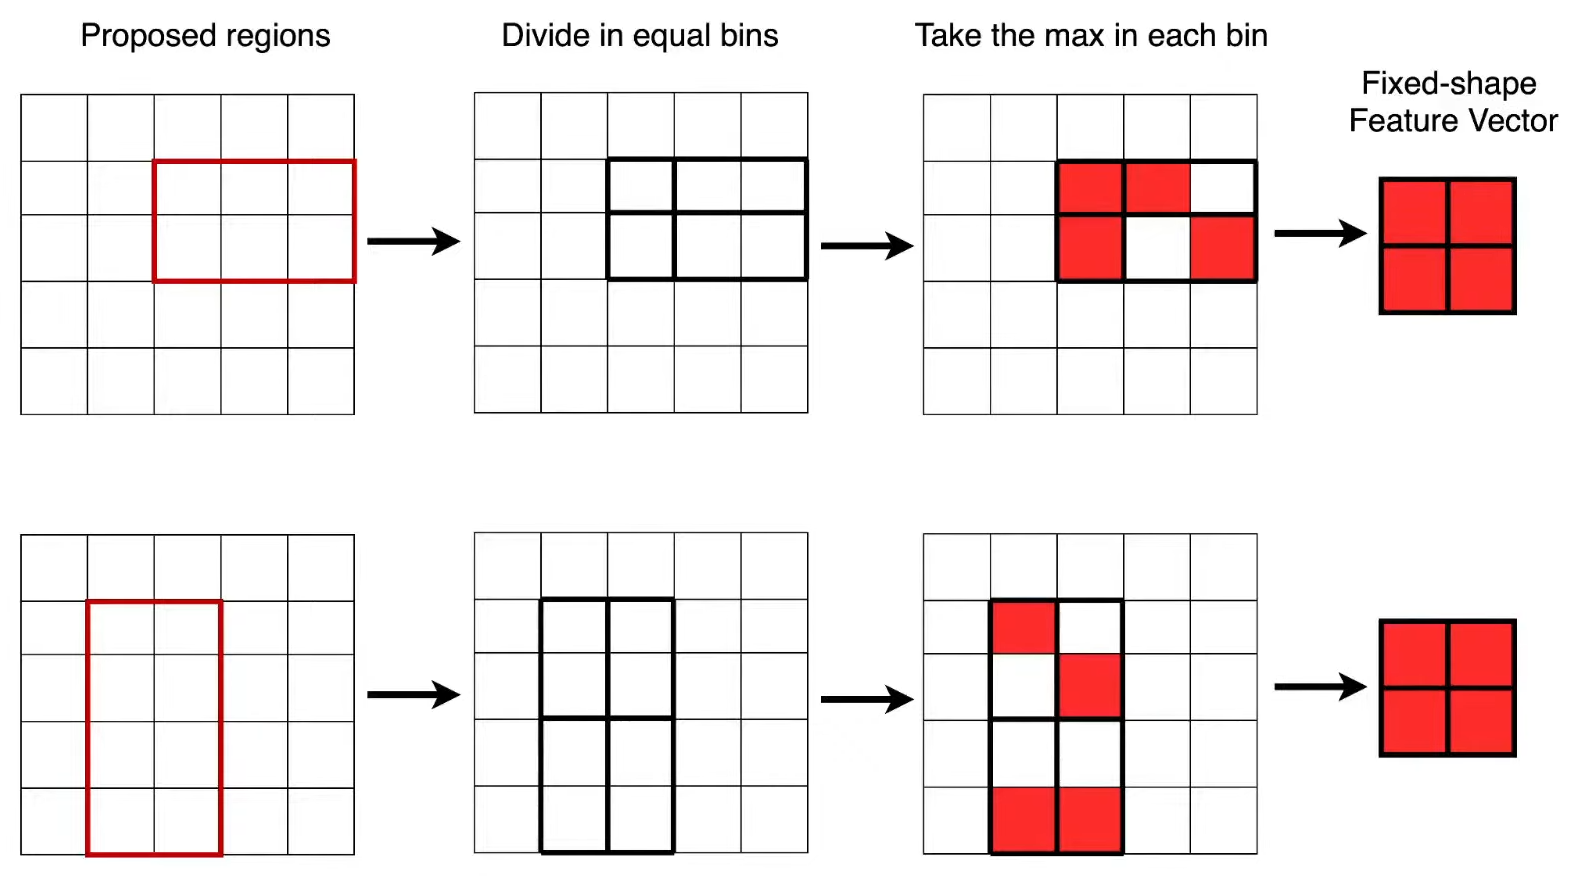
\includegraphics[scale=0.3]{img/roi_pooling.png} 
    \end{center}
    \item Then we take these fixed size feature vectors and feed them through a fully connected neural network to get a feature vector where we can do softmax classification on, along with regression of the bboxes dimensions. 
  \end{enumerate}

  \begin{center}
      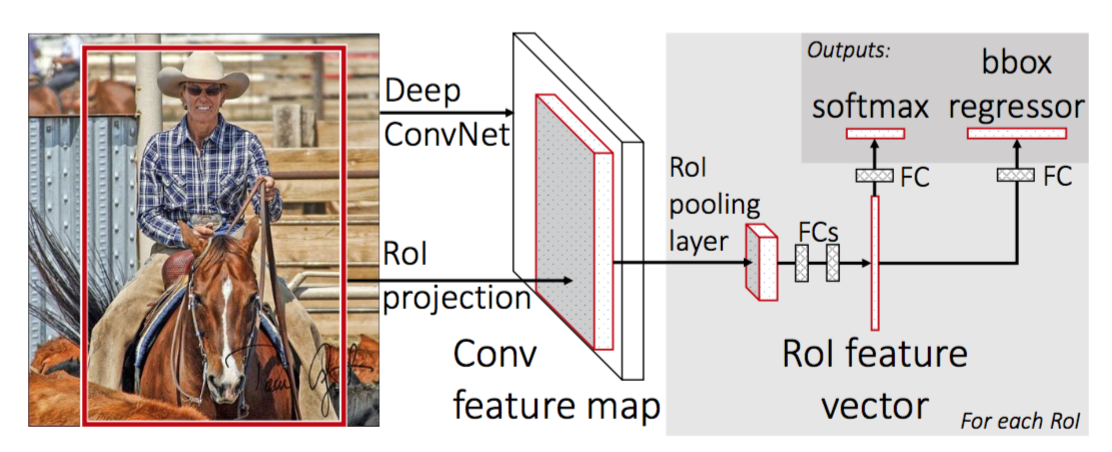
\includegraphics[scale=0.3]{img/fast_rcnn.png}
  \end{center}

  Regarding the problems, this first improves the computational cost compared to R-CNN. By utilizing the IOU pooling layers, we have resized the images after the CNN feature extractor rather than distorting the original input itself. Moreover, we have replaced the SVM classifiers with neural nets. However, we still have the problem that the region proposal algorithm is an external algorithm that's not learned, and this selective search method still turns out to be quite slow for real-time inference.  

\subsection{Faster RCNN}

  Therefore, Ren et al, came up with an object detection algorithm that eliminates the selective search algorithm and lets the network learn the region proposals. The Faster RCNN model essentially repalces the region proposal algorithm with a significantly faster neural network that can learn to propose better regions for the task at hand. 
  \begin{center}
      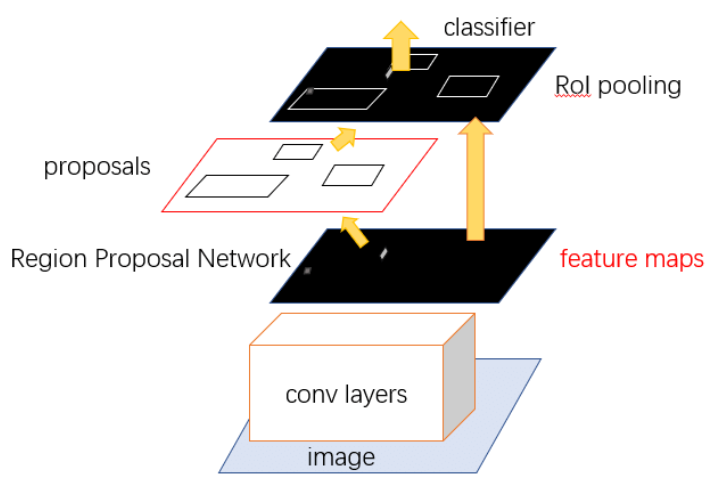
\includegraphics[scale=0.4]{img/faster_rcnn_diagram.png}
  \end{center}

  Let's walk through the steps of this algorithm: 
  \begin{enumerate}
      \item We take the image $\mathbf{x}$ and run it through a backbone convolutional network (usually the first few layers of ResNet or VGG), generating a feature map $\phi \in \mathbb{R}^{K \times K}$. There are $K^2$ ``points" or ``pixels" in this feature representation of $\mathbf{x}$, and \textbf{anchor points} are generated on $\phi$ . If they are projected back into the original image, we would have $K^2$ equally spaced points over $\mathbf{x}$. 
          \begin{center}
              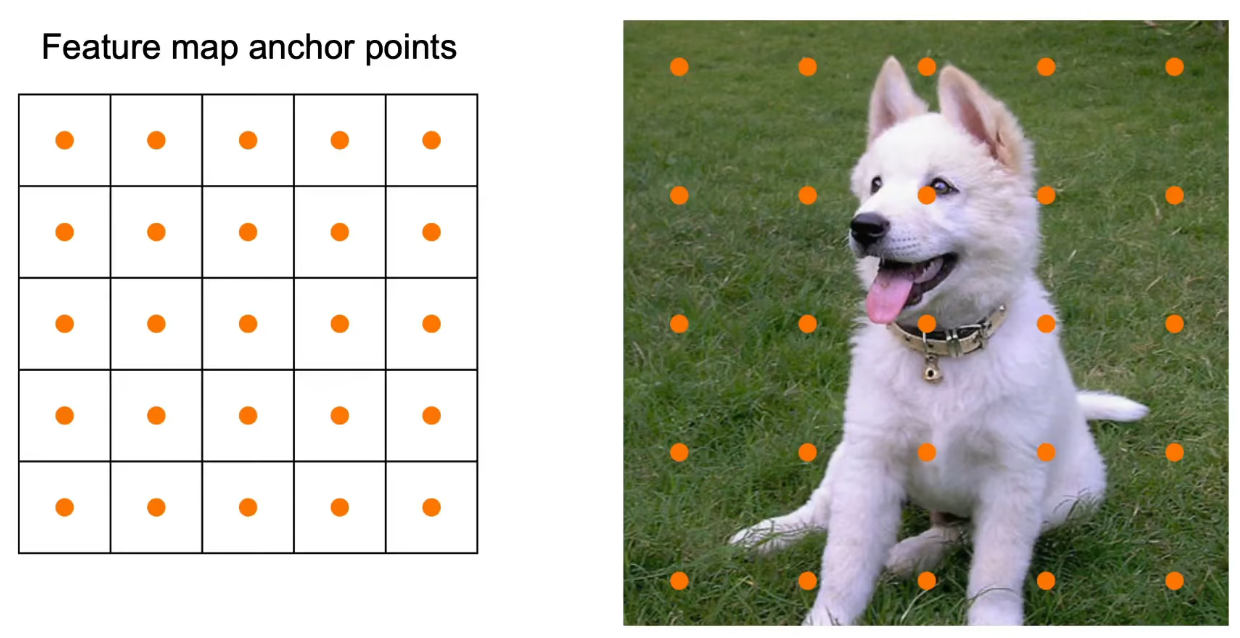
\includegraphics[scale=0.2]{img/anchor_points.png}
          \end{center}
      \item For each anchor point, we have $k$ predefined boxes of different sizes and aspect ratios that are used to generate region proposals that may or may not contain objects of interest. For example, we can have $k = 4$ in the picture below. 
      \begin{center}
          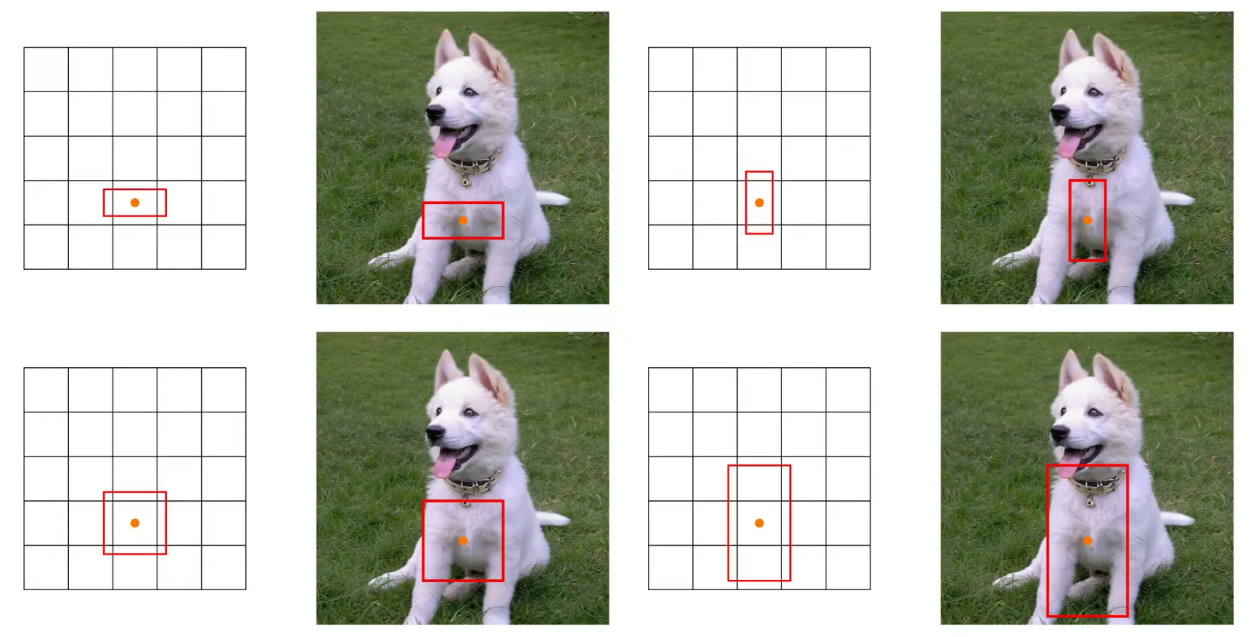
\includegraphics[scale=0.2]{img/anchor_boxes.png}
      \end{center}
      \item At this point, we have a total of $k K^2$ total anchor boxes on the feature space. We project all this back to the original image space, and we look for the samples that have a good IoU (calculated in the feature space with the projected ground truth boxes!) with the ground truth bbox. We generate (usually an equal amount) of positive and negative samples from the $k K^2$ total boxes. 
      
      \item For each of the $k K^2$ boxes, we want to classify each as an object or background, along with predicting their offsets from the corresponding gt bboxes. To do this, we use $1 \times 1$ convolutional layers. We take the feature map, which is of shape $(C, K, K) = (2048, 8, 8)$ and use the kernel to give us an output of size $(k, K, K)$. This output basically labels each of the $k K^2$ anchor boxes with some scalar that represents whether we think it is an object or background. We take a second $1 \times 1$ kernel and have it output $(4k, K, K)$ representing the offsets of the bounding boxes. This is called the regression head, and we need $4k$ since there are 4 degrees of freedom in adjusting each bounding box. 
      
      \item Now we have the scores and offsets of all the anchor boxes. But during training we only select the positive and negative anchor boxes to compute classification loss, and only positive boxes to compute the L2 regression loss. 

      \item In this second stage, we receive region proposals and predict the category of the object in the proposals. These region proposals (due to the anchor boxes being different sizes) are not the same size, so we use RoI pooling just like in Fast RCNN. After this, it's the same: we pass them through a fully connected MLP with some softmax and regressor link. 

      \item During inference, we pass the image through the backbone network to generate anchor boxes. Then, we select only the top ~300 boxes that get a high classification score and qualify them for the next stage. We then predict the final categories and offsets, performing an extra post-processing step called non-max surpression to remove duplicate bounding boxes. 
  \end{enumerate}

  Note that since we are using convolutions, this makes the object detection algorithm translationally invariant, and rotational invariance can be achieved through data augmentation. 

\subsection{Mask RCNN}

\subsection{Measuring Performance} 

  Recall that if we are just predicting the presence of 1 class, then we can talk about the recall or precision. A better way is to look at the mean precision, which is found by taking the integral of the precision recall curve. Other metrics include the $F_1$ score. 
  \[\text{Precision} = \frac{TP}{TP + FP}, \; \text{Recall} = \frac{TP}{TP + FN}, \; F_1 = 2 \frac{\text{Precision} \cdot \text{Recall}}{\text{Precision} + \text{Recall}}\]
  For multiple classes, we can use the \textbf{mean average precision}, which is basically the average precision for multiple classes.

  So far, we can use CNNs to either classify or regress an input image. However, the task of \textbf{object detection} requires us to draw bounding boxes around an arbitrary number of objects within an image \textit{and} correctly label each one. This seems like quite an enormous task, but we can build it up step by step. 

